\section{代理模型构建}

\subsection{候选模型谱系}

为建立赛车工况参数到稳定性评分的回归映射，
从传统回归到深度学习构建了6个模型的完整对比谱系：

\begin{enumerate}
    \item \textbf{M1 Ridge}（Ridge回归）：线性基准模型，
        提供模型复杂度下界的参考；
    \item \textbf{M2 Random Forest}（随机森林）：集成学习的经典代表，
        对噪声和过拟合有一定鲁棒性；
    \item \textbf{M3 XGBoost}：梯度提升决策树，
        以其在表格数据上的卓越表现著称；
    \item \textbf{M4 MLP}（多层感知机）：3隐藏层（128-256-128-64）
        的前馈神经网络，配备ReLU激活和Dropout正则化；
    \item \textbf{M5 TabNet}：基于注意力机制的可解释深度学习模型，
        专为表格数据设计；
    \item \textbf{M6 DeepEnsemble}（深度集成）：3个独立MLP的集成，
        仅改变初始化种子和数据shuffle。
        输出预测均值$\mu(x)$和标准差$\sigma(x)$，
        为风险敏感PSO提供不确定性估计。
\end{enumerate}

\subsection{训练配置}

MLP/DeepEnsemble采用以下训练配置：
\begin{itemize}
    \item 优化器：Adam（lr=$1\times10^{-3}$，weight\_decay=$1\times10^{-5}$）
    \item 损失函数：加权MSE（低稳定性样本权重加倍）
    \item 正则化：Dropout（p=0.2），Early Stopping（patience=20）
    \item 批量大小：256
    \item 最大训练轮数：500
\end{itemize}

为应对数据不平衡问题，
在损失函数中引入类平衡权重，
使模型对低稳定性样本的预测误差给予更高惩罚。

XGBoost采用以下配置：
\begin{itemize}
    \item 树数量：300
    \item 最大深度：6
    \item 学习率：0.1
    \item 子采样率：0.8
    \item 列采样率：0.8
\end{itemize}

\subsection{评价指标}

采用以下指标评估各模型性能：

\begin{equation}
    \text{MSE} = \frac{1}{n}\sum_{i=1}^{n}(y_i - \hat{y}_i)^2
    \label{eq:mse}
\end{equation}

\begin{equation}
    R^2 = 1 - \frac{\sum_{i=1}^{n}(y_i - \hat{y}_i)^2}
                    {\sum_{i=1}^{n}(y_i - \bar{y})^2}
    \label{eq:r2}
\end{equation}

\begin{equation}
    \text{MAE} = \frac{1}{n}\sum_{i=1}^{n}|y_i - \hat{y}_i|
    \label{eq:mae}
\end{equation}

\subsection{模型对比结果}

\begin{table}[H]
\centering
\caption{6模型性能对比}
\begin{tabular}{lrrrrr}
\toprule
模型 & R$^2$ & MSE & MAE & RMSE & 延迟 (ms) \\
\midrule
M1 Ridge & 0.6330 & 225.0046 & 12.3392 & 15.0002 & 0.034 \\
M2 RandomForest & 1.0000 & 0.0000 & 0.0006 & 0.0025 & 37.073 \\
M3 XGBoost & \textbf{0.9999} & \textbf{0.0312} & \textbf{0.0350} & \textbf{0.1767} & \textbf{0.242} \\
M4 MLP & 0.9994 & 0.3897 & 0.3882 & 0.6243 & 0.403 \\
M5 TabNet & 0.9997 & 0.2002 & 0.3602 & 0.4475 & 7.847 \\
M6 DeepEnsemble & 0.9995 & 0.3272 & 0.2712 & 0.5720 & 1.230 \\
\bottomrule
\end{tabular}
\end{table}

\begin{figure}[H]
\centering
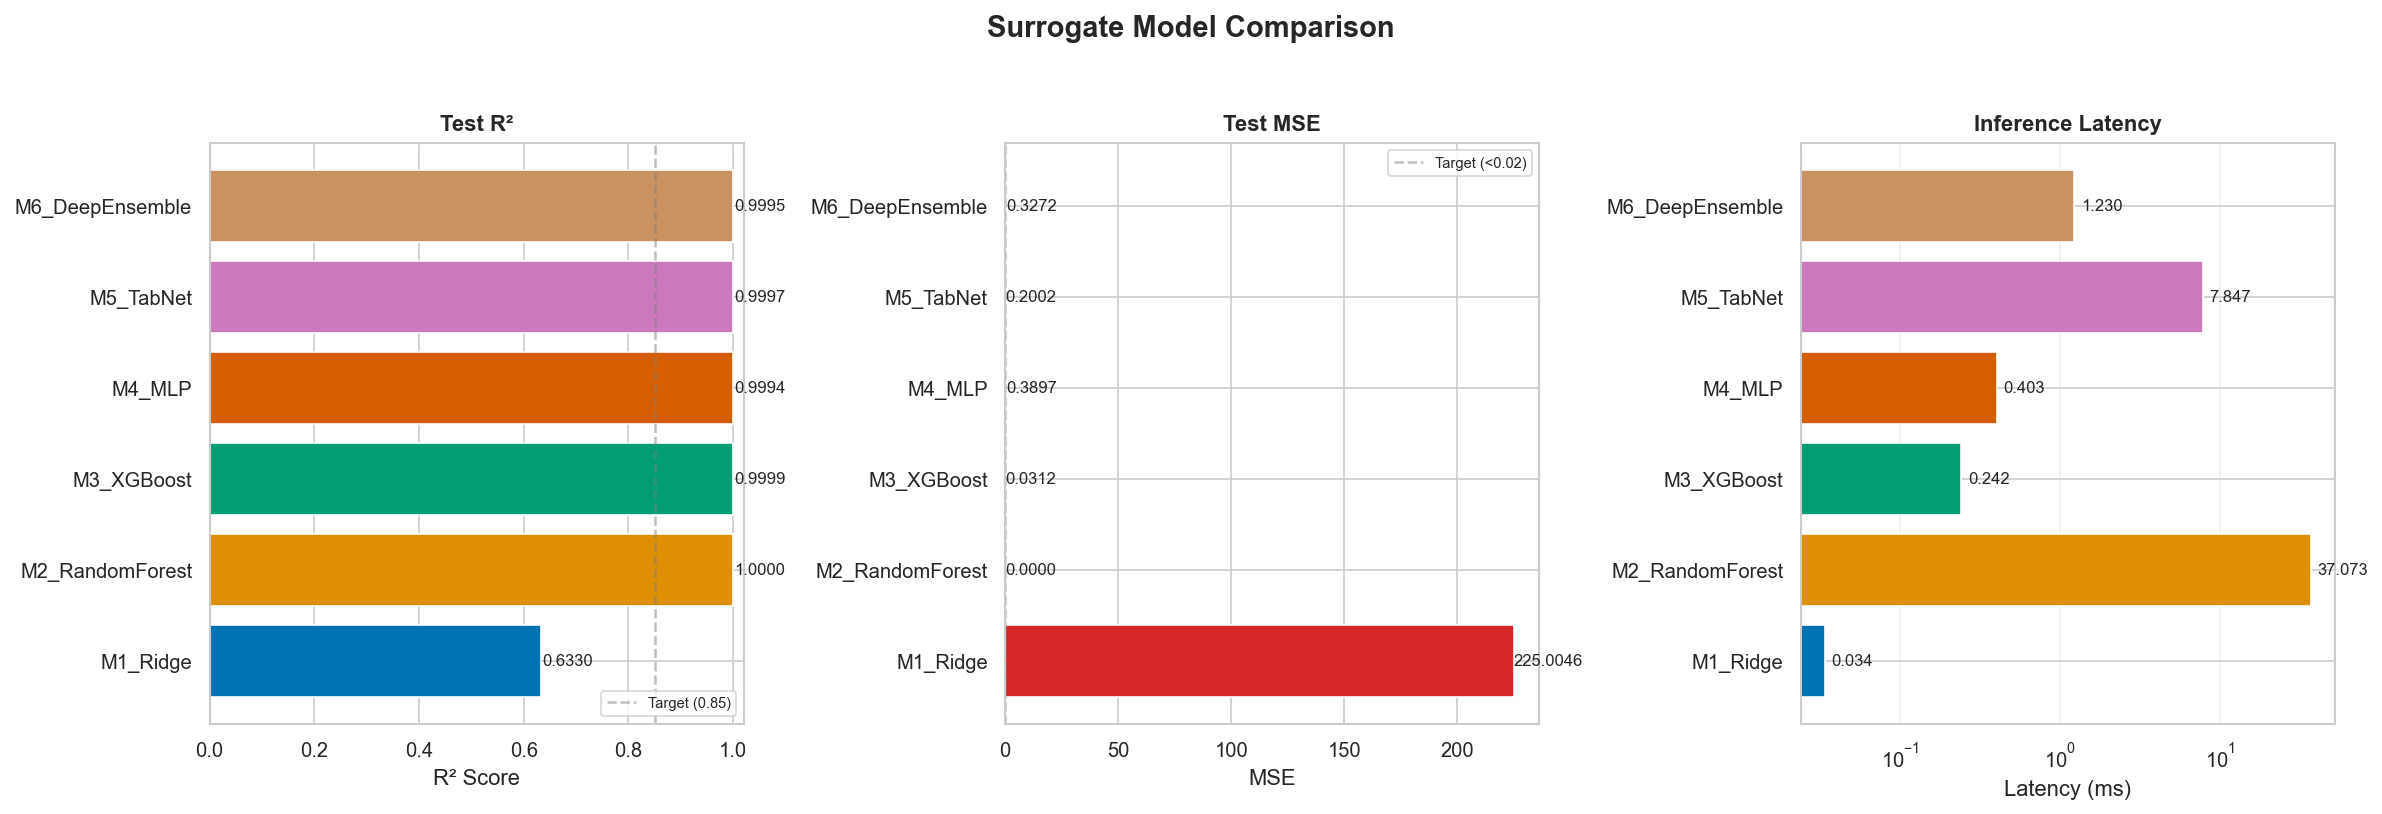
\includegraphics[width=0.80\textwidth]{figures/03_model_comparison.png}
\caption{6模型性能对比可视化（R$^2$、MSE、MAE、延迟）}
\label{fig:model_cmp}
\end{figure}

XGBoost（M3）在所有指标上均表现最优：
R$^2$ = 0.9999，MSE = 0.0312，MAE = 0.0350，
推理延迟仅0.242ms，完美适合PSO高频调用场景。
DeepEnsemble（M6）虽然精度略低于XGBoost
（R$^2$ = 0.9995，MSE = 0.3272），
但其不确定性估计能力$\sigma(x)$是风险敏感优化的关键组件。

Random Forest（M2）在测试集上达到R$^2$ = 1.0，
但37ms的推理延迟不适合PSO高频调用（每代50粒子$\times$80迭代
$\times$37ms $\approx$ 148s），
且存在过拟合风险。Ridge（M1）作为线性基准R$^2$仅0.633，
验证了该问题的强非线性特征。

\begin{figure}[H]
\centering
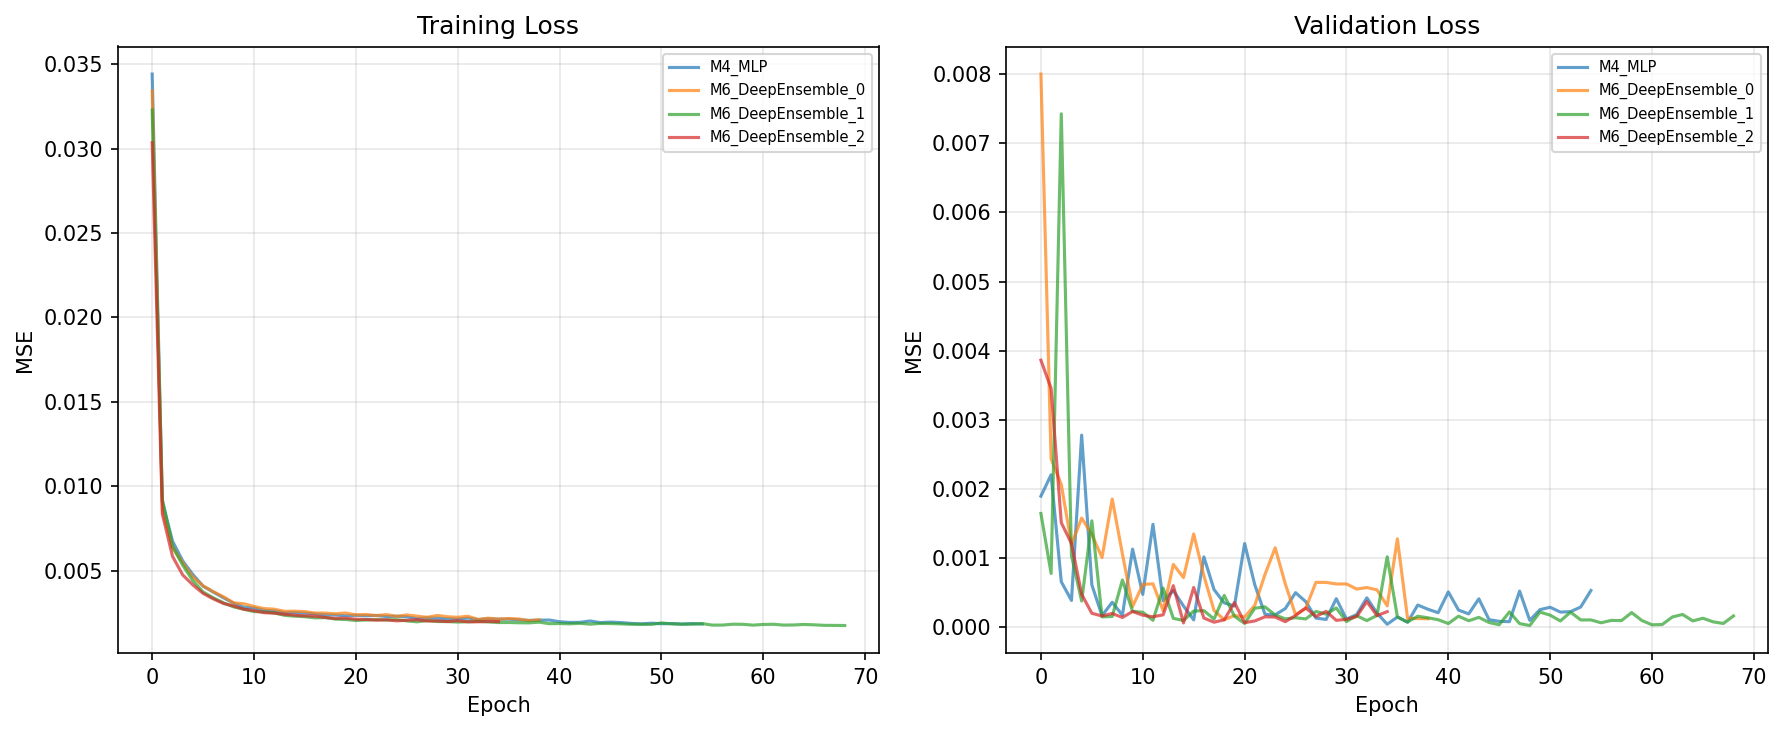
\includegraphics[width=0.78\textwidth]{figures/04_loss_curves.png}
\caption{神经网络模型训练损失曲线}
\label{fig:loss}
\end{figure}

图\ref{fig:loss}展示了MLP和DeepEnsemble的训练/验证损失随Epoch的变化。
MLP验证集MSE收敛至约0.39，DeepEnsemble的3个成员分别收敛至相近水平。
Early Stopping在约200轮时触发，防止了过拟合。

\subsection{模型选择策略}

基于精度-效率权衡：
\begin{itemize}
    \item \textbf{可解释性分析}（SHAP、排列重要性）：
        使用XGBoost（M3），
        因其TreeExplainer精确快速；
    \item \textbf{PSO寻优}：使用DeepEnsemble（M6），
        以提供$\mu(x)$和$\sigma(x)$用于风险敏感适应度计算。
\end{itemize}

\subsection{低稳定性样本的预测能力评估}

考虑到数据不平衡，
进一步评估各模型在低稳定性样本（stability\_index $< 95$）上的表现：

\begin{table}[H]
\centering
\caption{低稳定性样本上的模型表现}
\begin{tabular}{lrr}
\toprule
模型 & R$^2_{\text{low}}$ & MSE$_{\text{low}}$ \\
\midrule
M1 Ridge & 0.7815 & 239.0342 \\
M2 RandomForest & 1.0000 & 0.0000 \\
M3 XGBoost & 1.0000 & 0.0371 \\
M4 MLP & 0.9989 & 1.1690 \\
M5 TabNet & 0.9998 & 0.1725 \\
M6 DeepEnsemble & 0.9989 & 1.1494 \\
\bottomrule
\end{tabular}
\end{table}

XGBoost和Random Forest在低稳定性样本上继续保持极高精度，
MLP和DeepEnsemble略有下降但仍在可接受范围（R$^2_{\text{low}} \geq 0.9989$）。
这表明加权损失函数策略有效缓解了不平衡问题对模型拟合的负面影响。
